\section{Durchführung}
\label{sec:Durchführung}
Die Dampfdruckkurve wird anhand von Messungen im Bereich von $30\,\unit{\milli\bar}$ bis $1500\, \unit{\milli\bar}$ bestimmt.
Dafür werden die Messungen des niedrigen Bereichs (unter $1000\, \unit{\milli\bar}$) und des hohen Bereichs (über $1000\, \unit{\milli\bar}$)
mit zwei verschiedenen Apparaturen durchgeführt.
\subsection{Messbereich von $30\,\unit{\milli\bar}$ bis $1500\, \unit{\milli\bar}$}
\label{sec:ErsteDurchführung}
\begin{figure}[H]
    \centering
    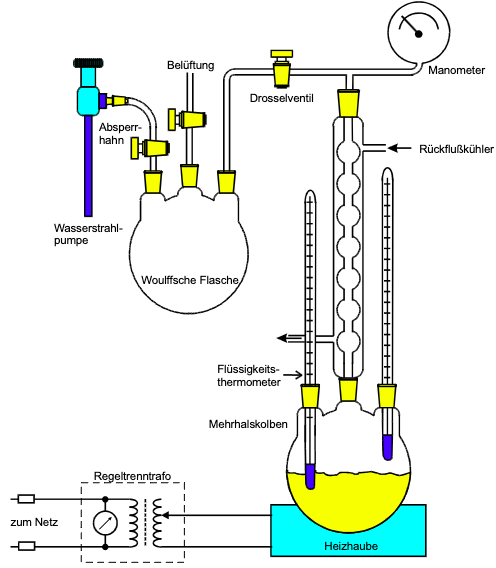
\includegraphics[width=0.90\textwidth]{Erste_Apparatur.png}
    \caption{Skizze der Messapparatur für den Druckbereich $p<1\,\unit{\bar}$. \cite{anleitungV203}}
    \label{fig:ErsteApparatur}
\end{figure}
\subsection{Messbereich von $1\,\unit{bar}$ bis $15\, \unit{\bar}$}
\label{sec:ZweiteDurchführung}
\begin{figure}[H]
    \centering
    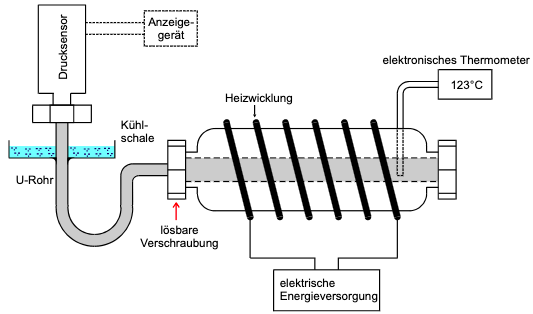
\includegraphics[width=0.90\textwidth]{Zweite_Apparatur.png}
    \caption{Skizze der Messapparatur für den Druckbereich $p>1\,\unit{\bar}$. \cite{anleitungV203}}
    \label{fig:ZweiteApparatur}
\end{figure}